\documentclass[10pt]{article}
\usepackage{icmlko}

\icmlmeta{IP 파운데이션 월드모델}{29}{4분의 3만 섞는다}{도메인 고유 축을 0.75배로 축소하면 축을 늘려도 정렬이 버틴다}

\begin{document}

\twocolumn[
\icmlheader

\begin{abstract}
노트 28은 축을 하나 더하는 것만으로 인자 기하가 회전해 정렬이 깨지는 것을 보고,
정렬 방법 대안을 미결로 남겼다. 두 방향을 시험했다. 먼저 극단 --- 도메인 고유
축을 공유 공간에 아예 넣지 않고 \textbf{교란 통제로만} 쓰는 부분 계수 전이다.
축 추가에 완전히 강건하지만(축을 켜도 $-$0.0535에서 $-$0.0537로 변화 없음)
성능이 낮다(유의 5, 평균 $-$0.0573 대 프로크루스테스의 $-$0.0762). 두 방법이
정보량과 안정성을 맞바꾸고 있으므로 사이를 이었다 --- 고유 축을 $\lambda$배로
축소해 공유 공간에 섞고 $\lambda$를 쓸었다. \textbf{$\lambda$=0.75가 답이다.}
게임 매장 노출도를 켜든 끄든 여섯 방향이 모두 유의하다($-$0.0691과 $-$0.0675).
$\lambda$=1.0은 축을 끄면 가장 좋지만($-$0.0762) 켜면 다섯으로 무너진다($-$0.0666).
문제는 고유 축의 존재가 아니라 \textbf{지배도}였다 --- 공유 축과 동등하게 섞으면
공간을 흔들고, 4분의 3으로 줄이면 정보는 남기고 흔들림은 사라진다. 부수적으로
구현 함정 하나를 기록한다 --- 상관행렬로 주성분을 뽑으면 $\lambda$ 축소가 표준화에
지워지므로 공분산을 써야 한다.
\end{abstract}
]

\section{두 극단을 먼저 재봤다}

노트 28의 문제는 이랬다. 게임에 매장 노출도를 넣으면 그 도메인의 인자 공간이
회전해 다른 도메인에서 온 계수가 맞지 않는다. 축 자체는 유용한데(게임이 출처일 때
개선) 정렬을 해친다.

원인은 구조에 있다. 인자 공간을 관측된 축 \emph{전부}로 만들고 그 공간을 회전으로
맞추므로, 축이 하나 늘면 공간 전체가 달라진다.

\subsection{극단 하나 --- 고유 축을 아예 넣지 않는다}

공유 축(타깃 폭, 굿즈 규모)만으로 공간을 만들고, 도메인 고유 축은 출처에서
\textbf{교란 통제}로만 쓴다. 즉 출처에서 y $\sim$ 공유 축 $+$ 고유 축을 적합하고
\emph{공유 축의 부분 계수만} 대상에 적용한다.

\begin{table}[t]
\centering\tsize
\caption{부분 계수 전이. 순열 3,000회.}
\begin{tabular}{lrr}
\toprule
구성 & 유의 방향 & 평균 차이 \\
\midrule
공유 축만 & 5 & $-$0.0573 \\
고유 축 통제 (매장축 끔) & 5 & $-$0.0535 \\
고유 축 통제 (매장축 켬) & 5 & $-$0.0537 \\
\midrule
{}[참고] 프로크루스테스 & 6 & $-$0.0762 \\
\bottomrule
\end{tabular}
\end{table}

\textbf{축 추가에 완전히 강건하다} --- 게임 매장 노출도를 켜도 $-$0.0535에서
$-$0.0537로 사실상 변화가 없다. 노트 28의 문제가 사라진다.

그런데 성능이 낮다. 프로크루스테스의 $-$0.0762에 견주면 25\% 약하고, 유의 방향도
다섯이다. 그리고 고유 축을 통제로 쓰는 것 자체는 이득이 없다($-$0.0573 $\to$
$-$0.0535로 오히려 조금 나쁘다).

이유는 분명하다. 프로크루스테스에서는 도메인 고유 축이 인자를 통해 공유 공간에
기여한다 --- 팝업의 다섯 축이 만든 두 성분이 옮겨지므로 다섯 축의 정보가 실린다.
부분 계수 방식은 그 경로를 막는다.

\claimx{프로크루스테스와 부분 계수는 정보량과 안정성을 맞바꾼다. 전자는 고유 축의
정보를 옮기지만 축 추가에 취약하고, 후자는 강건하지만 공유 축 둘의 정보만
쓴다.}{고유 축을 통제로 쓴 부분 계수가 프로크루스테스를 넘어서면 이 절충 자체가
없는 것이다.}

\section{사이를 이었다}

두 극단이 각각 $\lambda$=0(고유 축 배제)과 $\lambda$=1(고유 축 동등 혼합)에
해당한다. 고유 축을 $\lambda$배로 축소해 공유 공간에 섞고 쓸었다.

\begin{figure}[t]
\centering
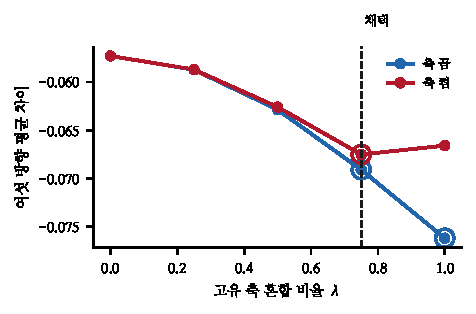
\includegraphics[width=\columnwidth]{figs/lam.pdf}
\caption{혼합 비율에 따른 성능. 빈 원이 여섯 방향 모두 유의한 점이다.}
\end{figure}

\begin{table}[t]
\centering\tsize
\caption{$\lambda$ 스윕. 순열 1,500회. 괄호 안이 유의 방향 수.}
\begin{tabular}{rrr}
\toprule
$\lambda$ & 게임 매장축 끔 & 게임 매장축 켬 \\
\midrule
0.00 & $-$0.0573 (5) & $-$0.0573 (5) \\
0.25 & $-$0.0587 (5) & $-$0.0587 (5) \\
0.50 & $-$0.0629 (5) & $-$0.0626 (5) \\
\textbf{0.75} & \textbf{$-$0.0691 (6)} & \textbf{$-$0.0675 (6)} \\
1.00 & $-$0.0762 (6) & $-$0.0666 (5) \\
\bottomrule
\end{tabular}
\end{table}

\begin{figure}[t]
\centering

\includegraphics[width=\columnwidth]{figs/sig.pdf}
\caption{유의 방향 수. $\lambda$=0.75에서만 두 구성이 모두 여섯이다.}
\end{figure}

$\lambda$=0.75가 유일하게 두 구성 모두에서 여섯 방향을 유지한다. $\lambda$=1.0은
축을 끄면 가장 좋지만($-$0.0762) 켜면 다섯으로 무너진다.

\claimx{도메인 고유 축을 0.75배로 축소해 공유 공간에 섞으면 축을 추가해도 정렬이
버틴다. 문제는 고유 축의 존재가 아니라 지배도였다.}{다른 도메인 조합이나 다른
축을 추가했을 때 0.75가 무너지면, 이 값은 현재 구성에 딸린 것이지 일반 상수가
아니다.}

\section{검증}

$\lambda$=0.75를 기본값으로 적용하고 순열을 3,000회로 올려 다시 쟀다.

\begin{figure}[t]
\centering

\includegraphics[width=\textwidth]{figs/six.pdf}
\caption{$\lambda$=0.75에서 게임 매장축을 켜고 끈 두 구성. 여섯 방향이 모두
유의하다.}
\end{figure}

\begin{table}[t]
\centering\tsize
\caption{$\lambda$=0.75, 순열 3,000회. 대상 라벨 미사용.}
\begin{tabular}{lrrrr}
\toprule
& \multicolumn{2}{c}{매장축 끔} & \multicolumn{2}{c}{매장축 켬} \\
방향 & 차이 & p & 차이 & p \\
\midrule
게임 $\to$ 아이돌 & $-$0.0931 & 0.0000 & $-$0.0922 & 0.0000 \\
팝업 $\to$ 아이돌 & $-$0.0842 & 0.0003 & $-$0.0842 & 0.0003 \\
게임 $\to$ 팝업 & $-$0.0784 & 0.0000 & $-$0.0807 & 0.0000 \\
아이돌 $\to$ 팝업 & $-$0.0683 & 0.0407 & $-$0.0683 & 0.0407 \\
팝업 $\to$ 게임 & $-$0.0477 & 0.0003 & $-$0.0466 & 0.0003 \\
아이돌 $\to$ 게임 & $-$0.0428 & 0.0107 & $-$0.0330 & 0.0393 \\
\bottomrule
\end{tabular}
\end{table}

두 구성 모두 여섯 방향이 유의하다. 축을 켜면 아이돌 $\to$ 게임이 $-$0.0428에서
$-$0.0330으로 약해지지만 유의성은 유지된다(p=0.0393).

\section{구현 함정 하나}

$\lambda$ 축소를 넣고 처음 돌렸을 때 고유값 분해가 발산했다. 원인은 주성분을
\emph{상관행렬}에서 뽑고 있었기 때문이다. 상관행렬은 각 열을 표준편차로 나누므로
$\lambda$ 축소가 그 단계에서 지워진다 --- $\lambda$=0에서는 축소된 열이 전부 0이
되어 분모가 0이 된다.

공분산행렬로 바꿔야 축소가 보존된다. 축 간 눈금이 이미 표준화돼 있으므로
공분산을 써도 특정 축이 지배하지 않는다.

\paragraph{기록해 두는 이유}
이 프로젝트에서 상관과 공분산을 바꿔 쓴 실수는 처음이 아니다. 노트 15에서
도메인마다 min-max로 정규화해 눈금이 어긋난 일이 있었다. 규칙으로 적어 둔다 ---
\textbf{가중을 넣은 뒤에는 표준화하지 않는다. 표준화가 가중을 지운다.}

\section{그래서 확정된 절차}

\begin{enumerate}[leftmargin=1.3em,itemsep=0.2em]
\item 도메인마다 관측 가능한 축을 잰다.
\item 공유 축은 그대로, 고유 축은 \textbf{0.75배}로 축소해 공분산 주성분을 뽑는다.
\item 공유 축의 적재로 기준 도메인에 직교 정렬한다(라벨 불필요).
\item 출처 도메인의 선형 계수를 대상에 적용한다.
\item 절대량이 필요하면 대상에서 8--20건을 실측해 중심과 중앙절대편차를 잡는다
      (노트 21).
\end{enumerate}

노트 19에서 확정한 파이프라인에 $\lambda$ 하나가 추가됐고, 그 대가로 축을
늘려도 정렬이 버틴다.

\section{한계}

\begin{itemize}[leftmargin=1.1em,itemsep=0.15em]
\item $\lambda$=0.75는 게임 매장 노출도 하나를 켜고 끄며 고른 값이다. 다른 축을
      추가할 때도 같은 값이 최적이라는 보장이 없다.
\item $\lambda$ 격자가 다섯 점뿐이다. 0.75와 1.0 사이에 더 나은 값이 있을 수 있다.
\item 축을 끈 상태만 보면 $\lambda$=1.0이 더 좋다($-$0.0762 대 $-$0.0691). 안정성을
      위해 9\%의 성능을 지불하는 선택이다.
\item 부분 계수 방식에서 고유 축 통제가 이득이 없던 이유를 규명하지 않았다.
\end{itemize}

\section{다음}

\begin{enumerate}[leftmargin=1.3em,itemsep=0.15em]
\item $\lambda$를 도메인별로 두는 방식 --- 축이 많은 도메인만 더 줄인다.
\item 입장 허들의 게임 측정 경로 --- 여전히 미해결.
\item 네 번째 도메인에서 $\lambda$=0.75 재확인.
\item 절대량 파이프라인을 $\lambda$=0.75 위에서 다시 측정(노트 21 갱신).
\end{enumerate}

\vspace{0.6em}
\hrule height 0.3pt
\vspace{0.5em}
{\footnotesize
\textbf{참고문헌}\\[0.3em]
Schönemann, P. H. (1966). A generalized solution of the orthogonal Procrustes
problem. \emph{Psychometrika}, 31(1), 1--10.\\[0.15em]
Hoerl, A. E., Kennard, R. W. (1970). Ridge regression: biased estimation for
nonorthogonal problems. \emph{Technometrics}, 12(1), 55--67.\\[0.15em]
Jolliffe, I. T. (2002). \emph{Principal Component Analysis}, 2nd ed. Springer.\\[0.15em]
Ben-David, S. et al. (2010). A theory of learning from different domains.
\emph{Machine Learning}, 79(1--2), 151--175.
}

\end{document}
